Small world networks are characterized by their very small characteristic path
length. With this in mind, one would see a very narrow range of values for
pairwise shortest path distances in a small world graph. DSD, however, is more
robust in that its range of possible values degrades more slowly as
characteristic path length increases.

In order to illustate this, we examined Watts-Strogatz graphs with various
values of $p$, starting from the regular ring lattice, $p = 0$. Histograms were
built by computing all of the pairwise distances in the graph using both
shortest path and DSD metrics. Notably, DSD experiences the same degradation as
shortest path distance for graphs with large p, ($p = 0.50$), which corresponds
to Watts-Strogatz graphs with low clustering coefficients, but is relatively
robust for $p = 0.10$, which is where clustering coefficients remain high. This
supports the intuition that DSD is an appropriate distance metric for graphs
that exhibit clustering and hub node behavior.

[These graphs are preliminary and I plan to replace them with density plots and
also to add scale-free networks in addition to performing a comparison on
summary statistics. -- JP]

\begin{figure}[!ht]
\centering
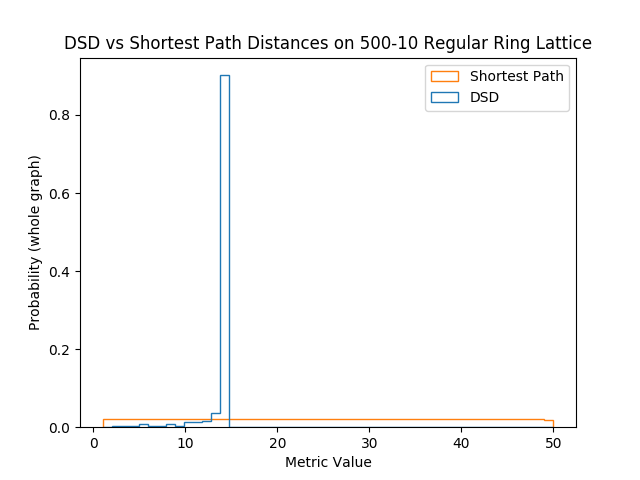
\includegraphics[width=0.85\textwidth]{hist_rrl.png}
\caption{}
\label{fig:hist_rrl}
\end{figure}

\begin{figure}[!ht]
\centering
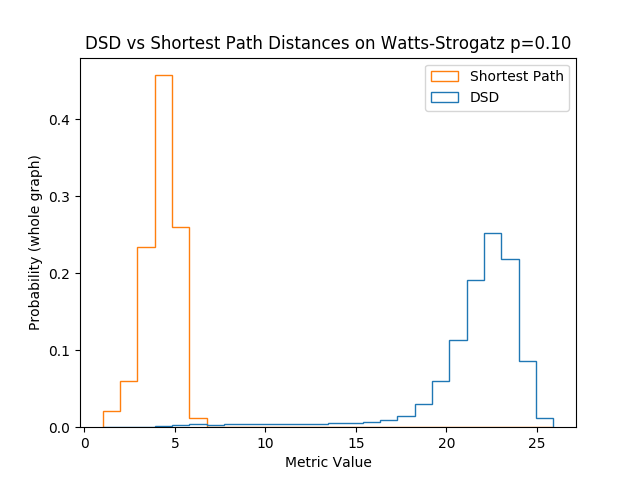
\includegraphics[width=0.85\textwidth]{hist_ws10.png}
\caption{}
\label{fig:hist_ws10}
\end{figure}

\begin{figure}[!ht]
\centering
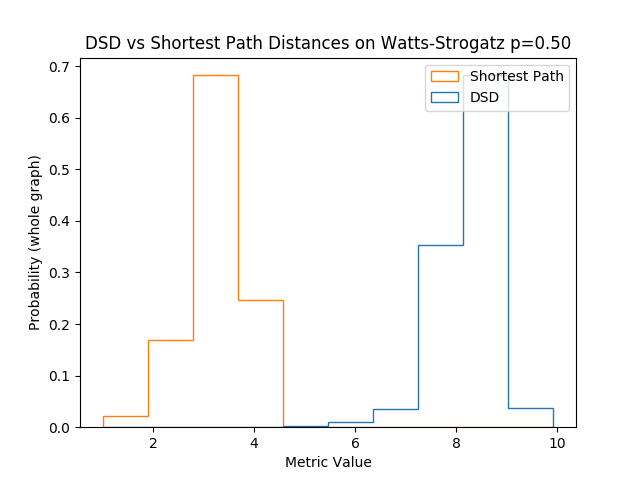
\includegraphics[width=0.85\textwidth]{hist_ws50.png}
\caption{}
\label{fig:hist_ws50}
\end{figure}
